\documentclass[twoside]{article}
\input{ISC18-english.sty}

\newcommand{\U}{\mathcal{U}}
\newcommand{\Sample}{S}
\newcommand{\GFS}{\mathrm{GFS}}
\newcommand{\OGFS}{\mathrm{OGFS}}
\newcommand{\NHT}{\mathrm{NHT}}
\newcommand{\Var}{\operatorname{Var}}
\newcommand{\pr}{\operatorname{Pr}}
\newcommand{\E}{\operatorname{E}}
\newcommand{\Crit}{\mathcal{C}}
\newcommand{\Leb}{\operatorname{Leb}}

\makeatletter
\setlength{\@fptop}{0pt}
\makeatother

\begin{document}
\thispagestyle{empty}

\fancyhead[LE]{Graphical Sampling with MCTS}
\fancyhead[RO]{Panahbehagh and Mohebbi}

\begin{center}
{
\includegraphics [height=25mm, width=\textwidth] {Images/isc18E}} \\
\vspace*{-1.8cm}
\vspace*{4cm}

{\Large \bf Graphical Finite-Population Sampling with Adaptive Monte Carlo Tree Search}\\

{\bf
Bardia Panahbehagh$^1$\footnote[1]{{\bf Corresponding Author:} {\tt bardia.panahbehagh@khu.ac.ir}},
Mehdi Mohebbi$^2$\\
$^1$Faculty of Mathematical Sciences and Computer, Kharazmi University, Tehran, Iran\\
$^2$School of Mathematics, Statistics and Computer Science, University of Tehran, Tehran, Iran}
\end{center}

\noindent\rule{\textwidth}{0.2mm}\par

\noindent{\bf Abstract:}\\
Graphical finite-population sampling represents prescribed first-order inclusion probabilities by bars, or unions of bar segments, on the unit interval. A horizontal uniform random line induces a sample, while the geometry of overlaps determines the second- and higher-order inclusion probabilities. Starting from the fixed-size graphical construction equivalent to Madow's systematic design, exchanges of interchangeable segments generate alternative fixed-size designs without changing the prescribed first-order probabilities. This paper combines that feasible design generator with an adaptive population-based Monte Carlo tree search. The implementation uses upper-confidence tree selection, quality-adaptive mutation scales, parallel two-scale rollouts, a safety cutoff, and restarts from the best design after stagnation. A tuning experiment based on the exact Narain--Horvitz--Thompson variance indicates that the restart and rollout mechanisms materially affect the quality of the best graphical design found.

\noindent{\bf Keywords:}
Finite-population sampling, graphical sampling, inclusion probabilities, Monte Carlo tree search, Narain--Horvitz--Thompson estimator. \\
\noindent{\bf Mathematics Subject Classification (2010):} $\rm 62D05$, $\rm 62K05$, $\rm 90C59$. \\
\noindent\rule{\textwidth}{0.2mm}\par

\section{Introduction}

Let $\U=\{1,\ldots,N\}$ be a finite population, and let
$\pi_k=\pr(k\in \Sample)$ be prescribed first-order inclusion probabilities
with $0<\pi_k<1$. Their sum is the expected sample size,
\[
    \sum_{k\in\U}\pi_k=\E(n_{\Sample}),
\]
and is denoted by $n$ when an integer fixed sample size is required. For a
study variable $y$, the Narain--Horvitz--Thompson estimator of the population
total $Y=\sum_{k\in\U}y_k$ is
\[
    \widehat Y_{\NHT}=\sum_{k\in \Sample}\frac{y_k}{\pi_k}.
\]
This estimator is design-unbiased whenever the prescribed first-order
inclusion probabilities are respected. Its variance, however, depends on the
second-order inclusion probabilities and therefore on the complete sampling
design. After fixing the vector $\pi$, the remaining problem is to construct a
feasible joint-selection structure that gives a small value of
$\Var(\widehat Y_{\NHT})$.

Graphical finite-population sampling (GFS), introduced by
\cite{Panahbehagh2026}, provides a visual and constructive representation of
this problem. Each $\pi_k$ is represented by a measurable bar set of total
length $\pi_k$ on the unit interval. Rearranging or exchanging bar segments
preserves the marginal inclusion probabilities but alters intersections among
bars, and hence changes the second- and higher-order inclusion probabilities.
The fixed-size version starts from a cumulative wrapped arrangement equivalent
to Madow's systematic sampling \cite{Madow1949}. Feasible segment exchanges
then generate a broad family of alternative designs with the same $\pi$ and
the same sample size.

This flexibility makes GFS a natural state space for intelligent design search.
The aim of this paper is to combine the fixed-size GFS mutation mechanism with
the adaptive multi-start Monte Carlo tree search (MCTS) implemented for the
{\tt graphical-sampling} package. The algorithm searches directly over feasible
graphical designs and evaluates them by the exact NHT variance. We first state
the graphical representation and its invariants, then describe the MCTS
implementation in a form aligned with the accompanying algorithm file, and
finally summarize its tuning experiment.

\section{Graphical Finite-Population Sampling}

\subsection{Graphical representation and exact design probabilities}

Let $B_k\subset[0,1)$ denote the bar set assigned to unit $k$. The bar may be
contiguous or may consist of several segments, but it must satisfy
\[
    \Leb(B_k)=\pi_k,
\]
where $\Leb(\cdot)$ denotes length. Draw $R\sim U(0,1)$ and define
\begin{equation}\label{eq:gfs-sample}
    \Sample(R)=\{k\in\U:R\in B_k\}.
\end{equation}
Therefore,
\[
    \pr(k\in\Sample)=\pr(R\in B_k)=\Leb(B_k)=\pi_k,
\]
so every graphical arrangement with the prescribed bar lengths has the desired
first-order inclusion probabilities.

\begin{figure}[ht]
\begin{center}
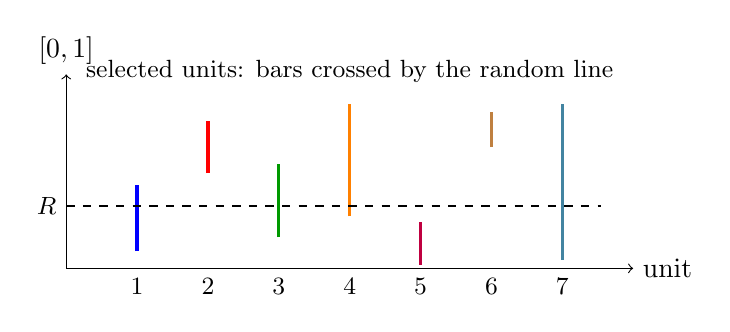
\begin{tikzpicture}[xscale=0.9,yscale=2.2]
  \draw[->] (0,0) -- (8,0) node[right] {unit};
  \draw[->] (0,0) -- (0,1.12) node[above] {$[0,1]$};
  \foreach \x/\a/\b/\c in {1/0.10/0.48/blue,2/0.55/0.85/red,3/0.18/0.60/green!60!black,4/0.30/0.95/orange,5/0.02/0.27/purple,6/0.70/0.90/brown,7/0.05/0.95/cyan!60!black}
    {
      \draw[very thick,\c] (\x,\a) -- (\x,\b);
      \node[below] at (\x,0) {\small \x};
    }
  \draw[dashed,thick] (0,0.36) -- (7.55,0.36);
  \node[left] at (0,0.36) {\small $R$};
  \node[above] at (4.0,1.02) {\small selected units: bars crossed by the random line};
\end{tikzpicture}
\caption{\footnotesize{A graphical sampling design. Unit $k$ is represented by
a bar set of length $\pi_k$. The horizontal line at $R$ selects all units whose
bars it intersects. The displayed bars are contiguous only for illustration;
a bar can be split into several segments after graphical mutations.}}\label{fig:gfs}
\end{center}
\end{figure}

The collection of all bar endpoints partitions the vertical axis into disjoint
strips $\Delta_1,\ldots,\Delta_D$. Within each strip the selected sample is
constant. Let
\[
    p_d=\Leb(\Delta_d),\qquad
    s_d=\{k:\Delta_d\subseteq B_k\},\qquad d=1,\ldots,D.
\]
Then $\sum_{d=1}^D p_d=1$, and the probability assigned to a distinct sample
$s$ is obtained by combining all strips that induce that same sample:
\begin{equation}\label{eq:design-law}
    p(s)=\pr(\Sample=s)=\sum_{d:s_d=s}p_d.
\end{equation}
Thus, the complete sampling design is known exactly from the graphical
arrangement. In particular, for any set $A\subseteq\U$,
\begin{equation}\label{eq:higher-order}
    \pi_A=\pr(A\subseteq\Sample)
    =\Leb\!\left(\bigcap_{k\in A}B_k\right)
    =\sum_{d:A\subseteq s_d}p_d.
\end{equation}
The second-order inclusion probabilities are the special case
\begin{equation}\label{eq:sip}
    \pi_{k\ell}=\Leb(B_k\cap B_\ell)
    =\sum_{d:k,\ell\in s_d}p_d.
\end{equation}
Consequently, the exact design variance of the NHT estimator is
\begin{equation}\label{eq:nhtvar}
    \Var(\widehat Y_{\NHT})
    =
    \sum_{k\in\U}\sum_{\ell\in\U}
    \frac{y_k y_\ell}{\pi_k\pi_\ell}
    \left(\pi_{k\ell}-\pi_k\pi_\ell\right),
\end{equation}
with $\pi_{kk}=\pi_k$. Different arrangements of the same bar lengths can
therefore have the same first-order probabilities but substantially different
precision.

An arbitrary GFS arrangement may have variable sample size and may produce many
zero second-order probabilities. These features motivate the fixed-size
construction and the segment-exchange operation described next.

\subsection{Fixed-size design generation by segment exchange}

Assume $\sum_k\pi_k=n\in\mathbb{N}$. The baseline fixed-size arrangement places
the bar lengths cumulatively on the unit interval, wrapping a bar around zero
whenever its upper endpoint exceeds one. This is the vertical graphical form of
Madow's systematic sampling. Every horizontal line then intersects exactly
$n$ bar segments, so $|\Sample(R)|=n$ for all $R$ except at endpoints of measure
zero.

Alternative fixed-size designs are generated by exchanging interchangeable
segments. Consider two strips $\Delta_i$ and $\Delta_j$ of heights $p_i$ and
$p_j$, inducing samples $s_i$ and $s_j$. Choose two substrips of common height
\begin{equation}\label{eq:vij}
    v_{ij}(\alpha)=\alpha\min(p_i,p_j),\qquad 0<\alpha\leq1.
\end{equation}
If there are units
\[
    k\in s_i\setminus s_j,
    \qquad
    \ell\in s_j\setminus s_i,
\]
then the segment of unit $k$ in the first substrip and the segment of unit
$\ell$ in the second substrip are interchangeable. Exchanging them splits the
two original strips and creates the modified samples
\[
    s_i^{k\leftrightarrow\ell}=(s_i\setminus\{k\})\cup\{\ell\},
    \qquad
    s_j^{k\leftrightarrow\ell}=(s_j\setminus\{\ell\})\cup\{k\}.
\]
Their probability masses are
\[
\begin{array}{c|cc}
 & \text{original sample} & \text{modified sample}\\ \hline
\Delta_i & p_i-v_{ij}(\alpha) & v_{ij}(\alpha)\\
\Delta_j & p_j-v_{ij}(\alpha) & v_{ij}(\alpha).
\end{array}
\]
Unit $k$ loses mass $v_{ij}(\alpha)$ in one strip and gains exactly the same
mass in the other; the same is true for unit $\ell$, while all remaining units
are unchanged. Hence all first-order inclusion probabilities are preserved.
Moreover, each modified sample replaces one unit by one unit, so the fixed
sample size is preserved. The operation changes bar intersections and therefore
changes $\pi_{k\ell}$ and the criterion in \eqref{eq:nhtvar}.

Repeated feasible exchanges define a local search mechanism over a large
family of graphical designs. In the software implementation, one call to
{\tt Design.iterate} applies such a graphical mutation. The arguments
{\tt switch\_coefficient} and {\tt random\_pull} control the mutation mechanism,
while the invariants---the vector $\pi$ and, for the fixed-size design, the
sample size---are maintained by the underlying GFS operation. This mutation is
the transition operator used by MCTS.

\section{Adaptive Population-Based Monte Carlo Tree Search}

Let $D$ denote a feasible graphical design and let
\[
    \Crit(D)=\Var_D(\widehat Y_{\NHT})
\]
be the criterion to minimize. More generally, the implementation accepts any
callable criterion. A tree node $v$ stores a design $D_v$, its parent and
children, the number of visits $N(v)$, the accumulated reward $Q(v)$, and the
mutation magnitude and type that produced it. The estimated node value is
\[
    \overline R(v)=\frac{Q(v)}{N(v)}
\]
when $N(v)>0$.

\subsection{Initialization, selection, and expansion}

The algorithm can start from a single design or a population
$D_1,\ldots,D_P$. For a population start, a virtual root is created and its
children contain the $P$ initial designs. The best initial criterion is
\[
    C_0=\min_{1\leq p\leq P}\Crit(D_p),
\]
and the corresponding design is stored as the incumbent best solution.

During traversal, an unvisited child is selected first. Otherwise, child $u$ of
node $v$ is selected by the upper-confidence score
\begin{equation}\label{eq:ucb}
    \operatorname{UCB}(u)
    =\overline R(u)
     +C\sqrt{\frac{\log\{\max(1,N(v))\}}{N(u)}},
\end{equation}
where $C>0$ is the exploration constant \cite{KocsisSzepesvari2006,Browne2012}.
Traversal continues while the current node has reached the allowed maximum
number of children.

Suppose a selected node at depth $d$ requires $b$ additional children. Three
mutation magnitudes are used:
\begin{align*}
    m_H &= \max(4,m_0),\\
    m_M(d) &= \max\!\left(2,\left\lfloor\frac{m_0}{2}\right\rfloor
                   -\left\lfloor\frac{d}{3}\right\rfloor\right),\\
    m_L &= m_{\min},
\end{align*}
where $m_0$ is {\tt base\_changes} and $m_{\min}$ is
{\tt min\_changes}. A child of type $q\in\{H,M,L\}$ is formed by copying the
parent design and applying {\tt Design.iterate} exactly $m_q$ times.

The allocation of the $b$ new children is quality-adaptive. If the node's mean
reward exceeds $0.5$, approximately $50\%$ of the children use low-magnitude
mutations, $20\%$ use middle-magnitude mutations, and the remainder use high
mutations. Otherwise, approximately $50\%$ use high mutations, $30\%$ use
middle mutations, and the remainder use low mutations. Thus, poorly performing
regions are explored more aggressively, whereas promising regions receive more
local refinement.

\subsection{Parallel adaptive two-scale rollout}

Every newly expanded child is evaluated by an independent rollout. The supplied
implementation performs $L=18$ rollout steps. Let $D^{(t)}$ be the current
rollout design, let $C^{(t)}=\Crit(D^{(t)})$, and let $\gamma$ denote the base
{\tt switch\_coefficient}. At each step, an aggressive candidate is generated
with
\[
    \gamma_A=\min(1,1.3\gamma).
\]
If it improves the current criterion, it is accepted. Otherwise, a conservative
candidate is also generated from the current design using
\[
    \gamma_B=\max(0.01,0.7\gamma),
\]
and the candidate with the smaller criterion among the aggressive and
conservative alternatives is accepted. This rule deliberately permits a
non-improving move when both alternatives are worse than the current state,
which gives the rollout a limited ability to cross local barriers. The best
design encountered during the rollout is retained separately.

A safety cutoff terminates the rollout whenever its current criterion exceeds
$1.15C_{\mathrm{ref}}$, where $C_{\mathrm{ref}}$ is the current reference
criterion. If $C_{\mathrm{roll}}^{\star}$ is the best criterion reached in the
rollout, the returned reward is
\begin{equation}\label{eq:reward}
    R=100\max\left\{0,
       \frac{C_{\mathrm{ref}}-C_{\mathrm{roll}}^{\star}}
            {C_{\mathrm{ref}}}\right\}.
\end{equation}
The rollouts for all newly created children are executed in parallel using the
available CPU cores, while the BLAS-related thread counts are fixed at one to
avoid nested parallelism.

\subsection{Backpropagation, incumbent update, and restart}

For each completed rollout, its reward is added to every node on the path from
the child to the root, and the visit count of each of those nodes is increased
by one. If the best design found in a rollout improves the global incumbent,
the incumbent design and criterion are updated and the iteration of the last
improvement is recorded.

The code also uses a stagnation restart, called a ``teleport'' in the
implementation. When more than three iterations have elapsed since the last
global improvement, the current tree is discarded and a new root is created
from the best design found so far. The reference criterion in
\eqref{eq:reward} is simultaneously reset to that incumbent value. The initial
population therefore supplies diversity at the beginning of the run, whereas
subsequent restarts intensify the search around the best available design.

\begin{alg}\label{alg:mcts}
Adaptive population-based MCTS for fixed-size graphical designs.
\begin{itemize}
\item Input one or more feasible GFS designs, a criterion $\Crit$, mutation
      parameters, an exploration constant $C$, an iteration budget, and a
      maximum number of children per node.
\item Evaluate the initial population, store the best design, and connect the
      initial designs to a virtual root.
\item Traverse the tree by \eqref{eq:ucb}, giving priority to unvisited nodes.
\item Expand the selected node with quality-adaptive high-, middle-, and
      low-magnitude sequences of feasible GFS segment exchanges.
\item Run the adaptive aggressive/conservative rollout for each new child in
      parallel; apply the $15\%$ safety cutoff and compute reward
      \eqref{eq:reward}.
\item Update the global incumbent and backpropagate the rollout reward.
\item After stagnation, replace the tree by a new root containing the incumbent
      best design and continue until the iteration budget is exhausted.
\item Return the best graphical design and its criterion value.
\end{itemize}
\end{alg}

\section{Simulation Results}

The simulation report studies the sensitivity of MCTS tuning parameters while
all other settings are fixed. The criterion is the exact NHT variance of the
current graphical sampling design, so smaller values are better. Unless a
parameter is being varied, the baseline settings are 150 iterations, population
size 10, eight children per node, 20 base changes, switch coefficient 1.0,
exploration constant 10, and 18 rollout steps. The current algorithm file uses
the selected rollout length 18, the safety factor 1.15, and a restart after more
than three iterations without a global improvement. The main findings are
summarized in Table \ref{tab:tuning}. The values shown are the best criterion
values reported among repeated runs for each tested setting and should be read
as algorithmic tuning results rather than inferential comparisons.

\begin{table}[ht]
\begin{center}
\footnotesize
\caption{Summary of the MCTS tuning experiment. Smaller criterion values are
better.}\label{tab:tuning}
\begin{tabular}{|p{3.2cm}|p{4.7cm}|p{2.0cm}|p{2.4cm}|}
\hline
Parameter & Tested settings & Best setting & Best criterion \\ \hline \hline
Maximum children per node & $5,8,10,15,20$ & $8$ & $163103.34$ \\ \hline
Base changes & $5,10,15,20,25$ & $20$ & $163103.34$ \\ \hline
Switch coefficient & $0.5,0.7,0.9,1.0$ & $1.0$ & $163103.34$ \\ \hline
Exploration constant & $0.5,1.5,5,10,15$ & $10$ & $163103.34$ \\ \hline
Rollout steps & $10,18,30$ & $30$ & $162093.85$ \\ \hline
Population size & $1,10,20,30,40$ & $10$ & $163103.34$ \\ \hline
Early stopping factor & $1.15,1.30,1.50,1.70$ & $1.15$ & $163103.34$ \\ \hline
Restart after no improvement & $3,4,5,8$ & $3$ & $131905.23$ \\ \hline
\end{tabular}
\end{center}
\end{table}

The most important numerical result is the effect of the restart parameter.
Using the aggressive restart setting associated with three non-improving
iterations reduced the best reported criterion to $131905.23$, compared with
$163103.34$ under the less aggressive baseline. This suggests that persistent
expansion of a stale subtree can be inefficient in the graphical-design search
space and that restarting from the incumbent may be more valuable. Because the
current code restarts when the elapsed count is greater than three, the actual
restart is triggered on the following iteration.

The maximum number of children controls the breadth of each expanded node. A
small value gives limited branching, whereas a very large value increases the
number of parallel rollouts without necessarily improving the incumbent. In
this experiment, eight children gave the best balance. The selected
{\tt base\_changes}=20 corresponds to the high mutation magnitude; the middle
magnitude decreases with tree depth and the low magnitude remains at
{\tt min\_changes}. This adaptive mixture helps combine broad changes with local
refinement.

The results favor a switch coefficient near $1.0$ and an exploration constant
of $10$ among the values tested. Increasing the rollout length from 18 to 30
produced a slightly smaller best criterion, but with additional computational
cost. The current implementation therefore uses 18 rollout steps as a practical
compromise. Overall, the results indicate that restart frequency, rollout effort,
and the balance between mutation scales are central tuning components of the
MCTS search.

\section*{Discussion and Conclusion}

GFS converts the design problem into a geometric search over bar-segment
arrangements. The exact design law follows from the vertical strips, and all
first-order probabilities remain fixed because each unit retains the same total
bar length. Starting from the Madow-equivalent fixed-size arrangement,
interchangeable-segment exchanges preserve both the prescribed $\pi$ and the
sample size while modifying the joint inclusion structure. The exact NHT
variance can therefore be evaluated after every mutation without Monte Carlo
approximation of the sampling variance.

The adaptive population-based MCTS uses this feasible mutation operator in a
search that combines initial population diversity, UCB-based traversal,
quality-dependent mutation magnitudes, parallel two-scale rollouts, and
incumbent restarts. The tuning results suggest that the search is particularly
sensitive to stagnation management. These findings are computational rather
than an optimality proof: the returned design is the best design found under a
finite search budget. Future work should use repeated experiments with common
computational budgets and compare MCTS with the greedy best-first OGFS search,
A* search, cube sampling, and determinantal sampling on larger simulated and
real populations.

\begin{thebibliography}{99}

\bibitem[Browne et al. (2012)]{Browne2012}
Browne C.B., Powley E., Whitehouse D., Lucas S.M., Cowling P.I., Rohlfshagen P., Tavener S., Perez D., Samothrakis S. and Colton S. (2012), A survey of Monte Carlo tree search methods, {\it IEEE Transactions on Computational Intelligence and AI in Games}, 4(1), 1--43.

\bibitem[Deville and Till\'{e} (2004)]{DevilleTille2004}
Deville J.-C. and Till\'{e} Y. (2004), Efficient balanced sampling: The cube method, {\it Biometrika}, 91, 893--912.

\bibitem[Horvitz and Thompson (1952)]{HorvitzThompson1952}
Horvitz D.G. and Thompson D.J. (1952), A generalization of sampling without replacement from a finite universe, {\it Journal of the American Statistical Association}, 47, 663--685.

\bibitem[Kocsis and Szepesv\'{a}ri (2006)]{KocsisSzepesvari2006}
Kocsis L. and Szepesv\'{a}ri C. (2006), Bandit based Monte-Carlo planning, {\it Proceedings of the 17th European Conference on Machine Learning}, 282--293.

\bibitem[Loonis and Mary (2019)]{LoonisMary2019}
Loonis V. and Mary X. (2019), Determinantal sampling designs, {\it Journal of Statistical Planning and Inference}, 199, 60--88.

\bibitem[Madow (1949)]{Madow1949}
Madow W.G. (1949), On the theory of systematic sampling, II, {\it Annals of Mathematical Statistics}, 20, 333--354.

\bibitem[Narain (1951)]{Narain1951}
Narain R.D. (1951), On sampling without replacement with varying probabilities, {\it Journal of the Indian Society of Agricultural Statistics}, 3, 169--174.

\bibitem[Panahbehagh (2026)]{Panahbehagh2026}
Panahbehagh B. (2026), Graphical finite population sampling, {\it Survey Methodology}, 52(1), 129--150.

\bibitem[Panahbehagh et al. (2025)]{GraphicalSampling2025}
Panahbehagh B., Mohebbi M., HosseiniNasab A.M. and Moghadam M.H. (2025), {\it graphical-sampling: A Python package for graphical finite-population sampling}, Python package.

\end{thebibliography}
\end{document}
